%%%%%%%%%%%%%%%%%%%%%%% file typeinst.tex %%%%%%%%%%%%%%%%%%%%%%%%%
%
% This is the LaTeX source for the instructions to authors using
% the LaTeX document class 'llncs.cls' for contributions to
% the Lecture Notes in Computer Sciences series.
% http://www.springer.com/lncs       Springer Heidelberg 2006/05/04
%
% It may be used as a template for your own input - copy it
% to a new file with a new name and use it as the basis
% for your article.
%
% NB: the document class 'llncs' has its own and detailed documentation, see
% ftp://ftp.springer.de/data/pubftp/pub/tex/latex/llncs/latex2e/llncsdoc.pdf
%
%%%%%%%%%%%%%%%%%%%%%%%%%%%%%%%%%%%%%%%%%%%%%%%%%%%%%%%%%%%%%%%%%%%


\documentclass[runningheads,a4paper]{llncs}

\usepackage{amssymb}
\setcounter{tocdepth}{3}
\usepackage{graphicx}
\usepackage{epstopdf}
\usepackage{subfig}
\usepackage{array}
\usepackage{xcolor}
\usepackage{float}

\graphicspath{{images/}}

\usepackage{url}
\urldef{\mailsa}\path|ary506@york.ac.uk|
\newcommand{\keywords}[1]{\par\addvspace\baselineskip
\noindent\keywordname\enspace\ignorespaces#1}

\begin{document}

\mainmatter  % start of an individual contribution

% first the title is needed
\title{Gamification of Software Modelling Learning}

% a short form should be given in case it is too long for the running head
\titlerunning{Gamification of Software Modelling Learning}

% the name(s) of the author(s) follow(s) next
%
% NB: Chinese authors should write their first names(s) in front of
% their surnames. This ensures that the names appear correctly in
% the running heads and the author index.
%
\author{Alfa Yohannis \and Dimitris Kolovos \and Fiona Polack} %FACP: I've added our names (it's conventional to include supervisors in the author list).  I'm not sure how they want author lists formatting, so you might need to edit.
%
\authorrunning{Gamification of Software Modelling Learning}
% (feature abused for this document to repeat the title also on left hand pages)

% the affiliations are given next; don't give your e-mail address
% unless you accept that it will be published
\institute{Department of Computer Science, University of York, York, United Kingdom\\
\mailsa\\}

%
% NB: a more complex sample for affiliations and the mapping to the
% corresponding authors can be found in the file "llncs.dem"
% (search for the string "\mainmatter" where a contribution starts).
% "llncs.dem" accompanies the document class "llncs.cls".
%

\toctitle{Lecture Notes in Computer Science}
\tocauthor{Gamification of Software Modelling Learning}
\maketitle

\begin{abstract}
Software modelling has a fundamental role in software engineering. However, it is perceived as relatively difficult for learners to develop the necessary abstraction skills to master the subject. Gamification is now flourishing as a popular strategy to engage learners. This research attempts to exploit gameful design as an innovative approach, used to create games that reinforce learners' mastery of software modelling by developing their abstraction skills. Our approach to gameful design brings together gamification development concepts such as design lenses and intrinsic skill atoms, and pedagogical design principles from several learning theories and models. The research follows the Design Science Research Methodology and exploits Model-Driven Engineering best practices. To date, the research has been developing an early prototype for learning software modelling through gamification. For evaluation, the effects of the artefact will be measured using longitudinal controlled experiments.
\keywords{software modelling, gamification, learning, abstraction}
\end{abstract}

\section{Introduction}
Software modelling is commonly perceived as a difficult subject since it requires a mastery of abstraction \cite{Borstler2012}. However, this subject has a fundamental and crucial role in software engineering education and practice. Failure to master this topic will affect the student’s abstraction capability in analysing and designing a real-world software. Weak software modelling will likely cause software engineering students to face difficulties completing their degrees, as most of the software engineering related subjects have a sense of intrinsic abstraction problems \cite{Kramer2007}. Students' perception of software modelling will affect their attitude towards software engineering today and their career paths in the future.

The problems of learning appropriate abstraction skills for software modelling is similar to problems in mathematics, where most of the concepts can only be accessed through symbolical representations \cite{Duval2006}. Abstraction also requires the students to perform information hiding, generalisation, approximation or reformulation, leaving out the irrelevant aspects but keeping the relevant ones, or separation from the concrete reality \cite{Saitta2013}. To overcome these challenges, we need to put more effort into designing delivering software modelling training, developing a more concrete and motivating presentation which can engage students and facilitate deep learning.

In recent years, the use of games or game elements for serious purposes other than leisure has drawn lots of attention. Gamification \cite{deterding2011game} and Serious Games \cite{Michael2005} have been viewed as solutions to motivational problems that emerge when users are required to engage in activites that they perceive as boring, irrelevant or difficult, e.g. Learning sorting algorithms \cite{Yohannis2015} or C-programming \cite{Ibanez2014}.

Therefore, the purpose of this research is to investigate and develop a gamification design framework that systematically and semi-automatically drives gamification design to produce better designed software modelling games. More precisely, this research aims to answer the following research questions that are derived from the purpose of this study:
\begin{enumerate}
\item Which processes, aspects, principles, or components of software modelling and their teaching and learning practices should be included?
\item What types of game elements and their roles that can deliver software modelling learning best? 
\item What kind of orchestrating framework is needed to design the interaction between, software modelling and game elements to produce a better software modelling gamification?
\item To what extent does gamification of software modelling improve engagement and motivation and improve learners’ performance?
\end{enumerate}

Due to the limitation of number of pages, this paper does not cover some interesting aspects of this research, such as the architecture of the artefact and the validation methods applied to evaluate models created by learners. 

\section{Related Works}
Several approaches attempt to bring software modelling into a more concrete presentation that can be easily understood by learners, ranging from didactic learning \cite{moisan2009teaching}, modelling tools utilization \cite{Akayama2013}, alternative communication channels and the use of modelling language \cite{Brandsteidl2011}, immersive visual modelling through virtual environment \cite{neubauer2003immersive}, software design studio \cite{Whittle2014}, project-based approach \cite{Szmurlo2007}, to code generation investigation \cite{schmidt2014teaching}. However, most of the approaches have weaknesses in motivating learners to engage continuously, frequently, and actively to learn software modelling, which is the important aspect impacting greatly on learning \cite{Naps2005}. To address lack of engagement, we investigate game-based learning, to learn or teach software modelling. This method provides students with a new way of learning software modelling, which is not only interactive but also engaging enough to keep them learning continuously. 

The use of game elements for a purpose other than leisure is called gamification \cite{deterding2011game}. Gamification design is still an ongoing challenge \cite{Deterding2013}, and, to date, there is no gamification design framework that particularly structures the design of software modelling gamification; a framework that integrates game specific domain into software modelling. Hence, this research aims to develop a gamification design framework of software modelling learning.

Most of the software related gamification studies available are related to software engineering in a larger context or to other aspects of software engineering, such as software implementation and project management, rather than software modelling in particular \cite{Pedreira2015}. After the literature exploration, only four works have been identified applied gamification for software modelling. None of these works addresses software modelling learning in general --- how learners can learn abstraction in modelling. Instead, they address specific topics such as activity diagramming \cite{Richardsen2014}, coupling and cohesion \cite{Stikkolorum2014}, and enterprise architectures \cite{Groenewegen2010} \cite{Ionita2015}. Most of the works also cover pedagogical aspect superficially or not at all and validation is restricted to a very limited number of users.

\section{Research Methods}
Since the output of this work is designed artefacts, we decided to utilise the Design Science Research Methodology (DSRM) \cite{peffers2007design} as our umbrella methodology. DSRM is selected because it provides a comprehensive high-level conceptual framework how to undergo a full-cycle research process. It also provides six activity guidelines for understanding, developing, executing, and evaluating design artefacts. The six activities are (1) problem identification and motivation activity, (2) definition of objectives for a solution activity, (3) setting of targets for a solution activity, (4) design and development activity, (5) demonstration and evaluation activities, and (6) communication. 

The high-level characteristics of DSRM mean that we can employ other research methods as the sub-methods in each activity. For example, we employ interviews, literature reviews, and discussion with experts as our methods in problem identification and motivation activity, as well as using Deterding's lens of intrinsic skill atoms \cite{deterding2015lens} to produce a gameful design in the design and development activity.

\begin{table}[H]
\caption{Design lenses (game elements) applied in the gamification design.}\label{Table001}
\begin{center}
    \begin{tabular}{ | p{3.2cm} | p {8.7cm} | }
    \hline
	\textbf{Lenses} & \textbf{Elements}\\    
    \hline
    Challenges & Onboarding, scaffolded challenge, varied challenge \\    
    \hline
    Goals and Motivation & interim goals, intrinsic rewards\\
    \hline
	Actions and Object & bite sized actions, limited choices, microflow, underdetermination, sensual \\
    \hline
    Feedbacks & Immediate, juicy, actionable, appeal to motives, glanceable, varied, graspable progress\\
    \hline
    \end{tabular}
\end{center}
\end{table}

\section{Gamfication Design}
To deliver a gameful experience while playing with the artefact, game elements have to be embedded into the artefact's design. Thus, Design Lenses and Skill Atoms \cite{deterding2015lens} are utilised to determine the required game elements as well as the game mechanics. The design of the levels of the game has a gradually increased difficulty as well as variety in its challenges, to expose learners to different kinds of domains, models, and diagrams. The onboarding game element is also planned to be implemented into the artefact to help learners familiar with the control system and the flow of the game. The software modelling game design will also utilise templates to help learners building models without having to start from scratch. The foundation model is already given. They only need to continue the model the meets certain objectives. The design of the cycle of the game mechanics is derived from Intrinsic Skill Atoms \cite{deterding2015lens}, which have six components that should be defined: motivation, goals, actions and objects, challenges, rules, and feedbacks.  



\begin{table}[H]
\caption{Skill Atoms applied in the gamification design.}\label{Table002}
\begin{center}
    \begin{tabular}{ | p{3.2cm} | p {8.7cm} | }
    \hline
	\textbf{Atoms} & \textbf{Description}\\    
    \hline
    Motivation & Master the modelling (solve problem, able to construct model) \\    
    \hline
    Goals & Create models that satisfy requirements \\
    \hline
	Actions and Objects & Construct model using diagrams, elements of a diagram, keywords, hints \\
    \hline
    Challenges & Satisfy requirements, meet objectives\\
    \hline
	Rules & Inherent rules in every model diagram, constraints, objectives\\
	\hline
	Feedbacks & completed objectives, model metrics, and motivating words\\
	\hline
    \end{tabular}
\end{center}
\end{table}

\section{Visual Modelling Editor}
To support developers in the design and customisation of gamification for software modelling learning --- the integration of game elements into its learning activities --- at a high level of abstraction and so as to automatically build the game generator, this research is developing a visual modelling editor using Eugenia, a GMF-based graphical model editors \cite{kolovos2015eugenia}. Currently, developers can use the editor to design the gamification of software modelling learning by defining its flows, levels, challenges, and objectives. In the future, this research plans to add more features, such as user-customised types of modelling and diagrams. 

\begin{figure}[htb]
\centering
\frame{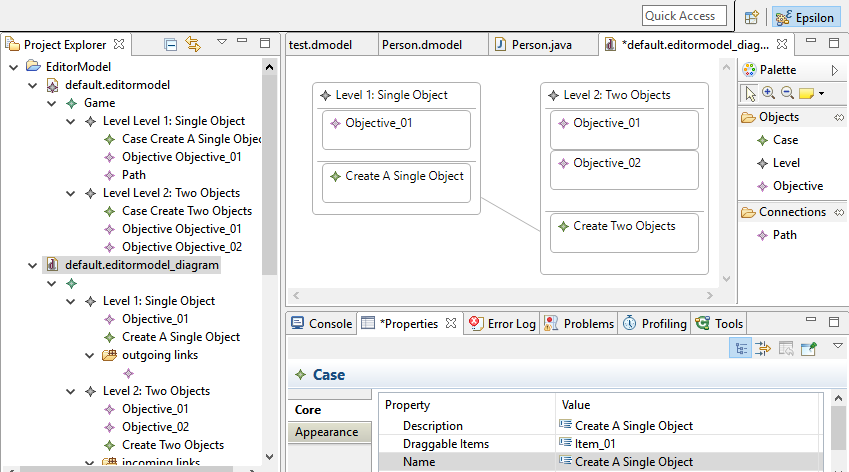
\includegraphics[width=11cm]{editor}}
\caption{Game editor to automatically generate the game.}
\end{figure}

\section{Evaluation}
The evaluation of the game artefact will use controlled experiments. The respondents, software modelling students, will be divided into two groups, a control group and experimental group. The control group will learn software modelling using traditional methods while the experimental group will learn with support from the artefact. After some time learning, both groups will be given problems to solve. Their performance will be measured by their ability to solve the problems. To anticipate the order effect, they will be asked to change their roles, from the control group to the experimental group and vice versa. After that, their ability will be tested again using similar problems. After the experiment, the significance of their performance will be calculated. To evaluate the generality of the effects of the artefact, a longitudinal experiment is also considered as well as undertaking the experiments in different countries and universities. Furthermore, The evaluation of the gamification design framework is similar to the game artefact's evaluation except for the respondents and problems will be software developers and software modelling gamification construction.

The controlled experiment is limited to measuring the significance of the design artefact. It cannot provide understanding to explain why learning software modelling supported with the artefact is better or worse than the traditional one. Consequently, surveying with questionnaires or interviews might be conducted to investigate the underlying variables or processes. Structural equation modelling \cite{hair2016primer} is also an option if measuring the effects of the identified underlying factors is required. An alternative method for understanding of underlying variables and processes is through investigating the artefact's event logs using data mining or machine learning techniques.

\section{Conclusion}
This paper explains our research motivation and problem statements, proposed solution and objectives, research methods, the current progress of the design and development of the artefact, and the evaluation plan. So far, this research is focusing its work on software modelling learning. In the future, this research plans to address metamodelling and model transformation learning. 

\subsubsection*{Acknowledgments.} Thanks to York Masters students who participated in our preliminary surveys. This research is supported by \emph{Lembaga Pengelola Dana Pendidikan Indonesia} (Indonesia Endowment Fund for Education). 

\begin{figure}[htb]
\centering
\frame{\includegraphics[width=11cm]{game-annotated}}
\caption{The game's display.}
\end{figure}

\bibliography{references} 
\bibliographystyle{ieeetr}

\end{document}


